%
% Complete documentation on the extended LaTeX markup used for Insight
% documentation is available in ``Documenting Insight'', which is part
% of the standard documentation for Insight.  It may be found online
% at:
%
%     http://www.itk.org/

\documentclass{InsightArticle}


%%%%%%%%%%%%%%%%%%%%%%%%%%%%%%%%%%%%%%%%%%%%%%%%%%%%%%%%%%%%%%%%%%
%
%  hyperref should be the last package to be loaded.
%
%%%%%%%%%%%%%%%%%%%%%%%%%%%%%%%%%%%%%%%%%%%%%%%%%%%%%%%%%%%%%%%%%%
\usepackage[dvips,
bookmarks,
bookmarksopen,
backref,
colorlinks,linkcolor={blue},citecolor={blue},urlcolor={blue},
]{hyperref}
% to be able to use options in graphics
\usepackage{graphicx}
% for pseudo code
\usepackage{listings}
% subfigures
\usepackage{subfigure}


%  This is a template for Papers to the Insight Journal. 
%  It is comparable to a technical report format.

% The title should be descriptive enough for people to be able to find
% the relevant document. 
\title{Optimization of connected component labelling}

% Increment the release number whenever significant changes are made.
% The author and/or editor can define 'significant' however they like.
%\release{0.00}

% At minimum, give your name and an email address.  You can include a
% snail-mail address if you like.
\author{Richard Beare}
\authoraddress{Department of Medicine, Monash University, Australia}

\begin{document}
\maketitle

\ifhtml
\chapter*{Front Matter\label{front}}
\fi


\begin{abstract}
\noindent
The report details some modifications made to the ITK 
{\em ConnectedComponentImageFilter} in an attempt to improve
performance. Some interesting observations were made during this
process. A new filter using a different algorithm to perform the same
function is also described and improved performance demonstrated.
\end{abstract}

\tableofcontents

\lstset{language=c++}
\maketitle
% \tableofcontents
\section{Introduction}
This work started out as my tutorial for writing ITK filters and
learning about iterators. 

The ConnectedComponentImageFilter performs a task known as {\em
labelling} in which each distinct object is given a unique
identifier\footnote{In practice this means that each pixel belonging
to a given object is given the same value} while the background is set
to zero. An object, or connected component, is usually defined as a
set of {\em connected}, non zero pixels, where two pixels being {\em
connected} means that it is possible to construct a path including
only non zero pixels between them. Steps along the path are defined by
a neighborhood function, as illustrated in Figure \ref{fig:neigh}\footnote{It
is feasible to have neighborhoods that include more than immediately
adjacent pixels, but this isn't done very often in practice}.

Labelling is often a pre-requisite for operations such as region based
intensity statistics and shape characterization. It is also useful
when using marker based segmentation approaches.

The connected component filter in itk has since been modified to
include a mask image. The modified filters do not include this
facility \footnote{It is not immediately clear why the masking
capability should be included in the filter rather than in the
pipeline preceeding it.}.

\begin{figure}[htbp]
\begin{center}
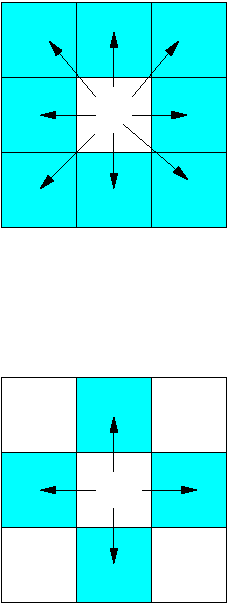
\includegraphics{connect}
\label{fig:neigh}
\caption{4 and 8 connected neighborhoods used in 2D labelling.}
\end{center}
\end{figure}

\section{Important notes}
Whenever optimizing itk filters there two important checks -- make
sure that you build the library in {\bf Release} mode. This is often
mentioned on the mailing lists, but is easy to forget. Release mode
isn't the default build option and makes a big difference in
performance when compared to the less optimized modes. Also ensure
that the ITK libraries are built with profiling turned on and that you
are linking against the correct libraries. If you built shared
libraries to support interpreter interfaces you may not be getting the
correct profile measurements. I discovered this much too late - in my
case much of the time related to the equivalency table was not
reported in my initial investigations.

\section{Current labelling algorithm}
The existing labelling algorithms is:
\begin{itemize}
\item Find all non zero input pixels and set the corresponding output 
pixel to the maximum label value.
\item Iterate over the output image. If the pixel is non zero, visit 
the neighbors of the pixel that have a lower index (the ``previous''
neighbor pixels).
\item If one or more of the previous pixels are already labelled 
then the current pixel will inherit a label from one of them.
\item If multiple neighors are labelled differently, then this 
information is inserted into the equivalency table.
\item Collapse the equivalency table after all output pixels have 
been checked.
\item Revisit all output pixels, lookup their value in the equivalency table and replace.
\end{itemize}

This is a 3 pass algorithm.

\section{Test hosts and images}
Two hosts were used to test the filter described in this report. The
first (host 1) was an AMD Athlon XP 2000+, 1.67GHz, 256kB cache and
256M RAM and the second (host 2) was an AMD Athlon 64 3000+, 1.8GHz
with 512kB cache and 1GB RAM.

Three images were used in testing, two of which are included in the
associated archive. The 2D image is the $217 \times 180$
BrainMidSagittalSlice image from the ITK distribution and the 3D
images are are a $371 \times 371 \times 34$ image of cells (ESCells,
included in the archive) and a $256 \times 256 \times 120$ brain mri
image that is not included in the archive. The ESCells image had about
twice as many pixels above the thresholds used in the study as the
brain mri image.

\section{Optimizing the existing filter}
The filter was optimized in two stages, and the timing results are
summarized in Tables \ref{tbl:timing1} and \ref{tbl:timing2}. The
first set of changed included:
\begin{itemize}
\item Updating the neighborhood iterator only when over non-zero pixels,
      rather than incrementing along with the standard iterator:
\begin{lstlisting}
nit += oit.GetIndex() - nit.GetIndex(); 
\end{lstlisting}

\item About 5\% of the computation time was being spent in the 
progress reporter. The reporter was modified to report once per stage,
rather than once per pixel. (This proportion was almost certainly
wrong, due to incorrect profiling).
\end{itemize}

%These changes lead to a reduction in computation time from {\bf 0.00477}
%to {\bf 0.00278} seconds for a face connected labelling of the
%BrainMidSagittalSlice image thresholded at 100 and from {\bf 1.06} to
%{\bf 0.922} seconds for the $371 \times 371 \times 34$
%ESCells image.

%A significant improvement for such a minor change in the first
%example! It should also be noted that as significant improvements were
%not observed in other 3D images that had a higher proportion of empty
%pixels, as would be expected.

The modified class is {\em itkConnectedComponentImageFilter1}.

The second attempt at optimization employed the approach recommended
in the ITK documentation -- avoid unnecesary boundary condition checks
by dividing the volume into regions using the face calculator. This
complicates the code, but doesn't change the fundamental
algorithm. The central volume is processed first, followed by the edge
volumes. Since we are no longer visiting the pixels in strict raster
order the neighborhood operators for the edge regions must visit all
neighbors, not just the ``previous'' ones, which probably means that
the equivalency table will be slightly larger than the original.



The modified class is {\em itkConnectedComponentImageFilter2}.

\subsection{Optimization results}
A curious thing to note is that the performance of both hosts was very
similar, despite one being a much older machine. It may be that the
performance of this type of operation is largely governed by memory
performance, and both machines have similar capabilities in this
regard.

The first modification produced a marked improvement in speed on
images that were largely empty, and will make no difference at all to
images that are completely full. This reasons are fairly obvious as we
have removed an operation that is redundant for empty pixels.

The second modification is somewhat harder to understand. For host 1
there was a minor improvement in the 2D case and the ESCells case, but
a decrease in performance in the case of the brain MRI. For host 2
there was no significant difference in the 2D case, a minor
improvement in the case of ESCells and a decrease in performance in
the case of the brain MRI.

It is difficult to be certain of the reason for this, but I suspect
that it relates to the cache performance. The 2D image is small enough
to fit in cache, so it doesn't matter very much whether the pixels are
visited in raster order or not. The brain mri image doesn't fit in
cache, so visiting face pixels that aren't in raster order may result
in a significant overhead that offsets any saving due to removal of
boundary condition check. If this hypothesis is
correct\footnote{Someone with the intel tools, like vtune, may be able
to check this.} then it demonstrates that the tradeoffs that must be
considered when optimizing filters are quite complex. This is
discussed in more detail in Section \ref{sect:performance_lessons}.

\section{A new labelling algorithm}
Further optimizations to the existing algorithm that avoid the need
for boundary checks are possible, but require dimension specific code,
which is not really the ITK way.

I've been considering an alternative, based on run length encoding,
that sidesteps many of these problems. The new algorithm proceeds as follows:
\begin{itemize}
\item Traverse each line of the input image (using a line iterator).
\item Build a data structure representing a run length encoded version
 of the line (each line will be a collection of {\em runs}. This is
 typically quite efficient because the input has only two values -
 zeros and non zeros, and we are usually interested in labelling
 ``blob'' like objects. Each run length is given a unique label.
\item Place the line data structure into a map.
\item Iterate through the map and find overlapping runs. Insert labels 
of overlapping lines into the equivalency table.
\item Collapse the equivalency table.
\item Iterate through the map, marking the output pixels with the appropriate values from the equivalency tables.
\end{itemize}

The advantages (in theory) of this approach are - only two passes over
images - one over input and the other over the output image. There are
no neighborhood operations requiring boundary checks. The equivalent
operations are performed on a per line basis using the map or when
searching for overlapping runs. In addition the check for equivalent
labels is done on a per run basis rather than a per pixel basis. The
differences between full connectivity and face connectivity should
also be less significant because the relevant checks are also done on
a per line basis.

There are some images that could produce extremely bad performance for
this algorithm -- labelling thin linear objects oriented orthogonal to
the direction of the line iterator is one example. However this is
fairly unlikely.

The code for this class is {\em itkConnectedComponentImageFilter3}
\footnote{Further improvements may be made by using line iterators
that don't maintain the index - indexes are used in this code, but not
particularly often so non indexed iterators may provide an advantage.}.

A progress reporter has been added to this filter to report progress
per line, rather than per pixel is normal. This is a compromise
between the standard per pixel approach and the per stage approach
adopted based on erroneous profiling information.

The performance figures for this approach show improvements in both
the 2D and 3D cases for both hosts. In some cases the improvement is a
factor of 10 over the original algorithm.

The trick that was necessary to guarantee this performance was to take
the opportunity to relabel without referencing the equivalency table
where ever possible. If this wasn't done the equivalency table proved
to be a bottle neck for some images.

\begin{table}[htbp]
\centering
\begin{tabular}{|c|c|c|c|}
\hline
Method & BrainMidSagittalSlice & brain mri & ESCells \\
\hline
\hline
0 - face conn & 0.00489   & 0.98 & 0.984 \\
0 - full conn & 0.005     & 1.51 & 2.84 \\
\hline
1 - face conn & 0.00288   & 0.517 & 0.789 \\
1 - full conn & 0.00287   & 0.819 & 2.54 \\
\hline
2 - face conn & 0.00265   & 0.589 & 0.754 \\
2 - full conn & 0.00247   & 0.949 & 2.33 \\
\hline
3 - face conn & 0.00103   & 0.19 & 0.083 \\
3 - full conn & 0.00104   & 0.212 & 0.09 \\
\hline
\end{tabular}
\caption{Execution time for host 1. \label{tbl:timing1}}
\end{table}

\begin{table}[htbp]
\centering
\begin{tabular}{|c|c|c|c|}
\hline
Method & BrainMidSagittalSlice & brain mri & ESCells \\
\hline
\hline
0 - face conn & 0.00392   & 0.94 & 1.08 \\
0 - full conn & 0.00367   & 1.46 & 3.21 \\
\hline
1 - face conn & 0.00277   & 0.595 & 1.0 \\
1 - full conn & 0.00241   & 0.928 & 2.94 \\
\hline
2 - face conn & 0.00278   & 0.665 & 0.925 \\
2 - full conn & 0.00235   & 1.12 & 2.85 \\
\hline
3 - face conn & 0.00087   & 0.218 & 0.103 \\
3 - full conn & 0.00087   & 0.239 & 0.071 \\
\hline
\end{tabular}
\caption{Execution time for host 2. \label{tbl:timing2}}
\end{table}

\section{Testing}
We need to test whether two labelled images are equivalent, rather
than whether every pixel is equal. A labelling filter is free to
assign any label it chooses provided they are unique and the
definition of ``connectedness'' is consistent. A new comparison
procedure has been written to support this.

Equivalence tests can be run using ``ctest'' as usual. Timing tests
will be run at the end of the equivalance tests, and can be run
separately using the runTimer2d.sh and runTimer3d.sh scripts, which
produce log files called timing2d.log and timing3d.log.

\section{Performance lessons}
\label{sect:performance_lessons}
Optimization of imaging algorithms is difficult to do well. A lot of
the commonly used procedure probably don't give a meaningful measure
of how an algorithm will perform in an application. However optimizing
is still worth doing and can lead to important insights and new
ideas. The important thing is to think of optimization as you might
any other experiment and consider exactly what it is you are testing.

Here are some thoughts.

Optimization of image related operations is very strongly dependent on
cache performance. Techniques that appear to offer very good
performance when tested on images that fit in cache may perform very
badly on images that don't - algorithms that access data in a semi
random way are examples. In the case of simple algorithms the
performance may be entirely dependent on the main memory
bandwidth. Some experiments I once did using the Intel SIMD
instructions illustrated this. When using SIMD instructions to perform
arithmetic on arrays it is theoretically possible to achieve
performance improvements of between 2 and 16 times, depending on the
data types involved. I used the gcc extensions that support vector
operations to implement SIMD array arithmetic, and when the arrays
were small the improvement in speed was obvious. However as soon as
the arrays became significantly larger than cache, the performance
became identical to the non SIMD equivalent. This was an example of
performance being entirely memory bandwidth dependent.

The streaming architecture used in ITK is potentially ideal for
optimizing cache performance. In the case of simple arithmetic, for
example, it would make sense to perform all of the operations on a
small block at a time and the move on to the next one. The problem is
that there are remarkably few interesting imaging algorithms that can
be broken up this way and probably even fewer applications that can be
constructed using only streamable filters.

The testing methodology is also open to question. For example, if we
test on a filter on a small image because the application is also
going to involve small images, then the usual procedure is to repeat
the computation a number of times and take the average. Sounds
reasonable. However most applications have quite a few steps, each of
which involves one or more copies of the image, so even with small
images we are likely to exceed the cache size. This means that
performance of filters that were measured by repeatedly running the
computation in cache are probably not going to resemble the
performance of filters in the application, because the application
only uses each image once or twice and needs to maintain multiple
copies of related images that consume cache resources.

In matrix libraries the size of operands is taken into account when
deciding how to carry out an operation. This leads to much more
complicated code, which is something that should probably be avoided
in ITK.

\section{Other observations}
None of the filters allow a connectivity of 18 for 3D images. The
commonly used connectivities in 3D are 6 (face connected), 26 (fully
connected) and 18. If the connectivity cube is considered as 3 layers
then for a connectivity of 18 the top layer has 5 active connection
(center and 4 corners), as does the bottom layer. The middle layer has
all elements active. I doubt that this capability is particularly
signficant, but it is worth noting that it isn't available.

\section{Conclusions}
The report has outlined some simple changes that can improve the
performance of the connected component image filter and introduced a
new implementation based on run length encoding that increases the
performance by a factor of 10 in some cases.

\bibliographystyle{plain}
\bibliography{InsightJournal}
%\bibliography{Article}
\nocite{ITKSoftwareGuide}

\end{document}

